\documentclass[12pt,a4paper]{report}
\footskip = 1cm

\usepackage{cmap}
\usepackage{type1ec}
\usepackage[T2A]{fontenc}
\usepackage[utf8]{inputenc}
\usepackage[russian]{babel}
\usepackage{pgffor}
\usepackage{calc}
\usepackage{fmtcount}

\usepackage{amsmath,amstext,amssymb,amsthm}
\usepackage{fullpage}

\usepackage{ifpdf}
\ifpdf
  \usepackage[pdftex]{graphicx}
  \usepackage[pdftex,unicode,bookmarks=false]{hyperref}

  \pdfminorversion=5
  \pdfcompresslevel=9
  \pdfobjcompresslevel=9
\fi

\pagestyle{empty}

\graphicspath{{./figures/}}

\DeclareMathOperator{\EX}{\mathbb{E}}

\renewcommand{\thesection}{\arabic{section}}
\renewcommand{\thesubsection}{}

% Константа
\def\const{\mathop{\mathrm{const}}\nolimits}

% Модуль
\providecommand{\abs}[1]{\left\lvert{#1}\right\rvert}


\newtheorem*{definition}{Определение}
\newtheorem*{example}{Пример}
\newtheorem*{property}{Свойство}
\newtheorem*{problem}{Задача}

\begin{document}




\chapter*{Data Structures}

\section*{Arrays}

{\bf Массив} -- структура данных, хранящая фиксированное число элементов одинакового размера, смежно расположенных в непрерывном куске памяти.

Требование одинакового размера элементов (обозначим его как $S$) здесь существенно, поскольку позволяет находить адрес $i$-го элемента по смещению от начала массива:
$$A_n = A_0 + S \cdot i$$
Таким образом, получение элемента массива по индексу занимает $O(1)$. 

\subsection*{Multidimensional Arrays}

Количество индексов, определяющих элемент в массиве, называется {\em размерностью} массива. Например, матрицу можно представить массивом размерности 2. При этом её элементы выстраиваются в линейный порядок по строкам ({\em row-major}, наиболее популярный, используется в частности в C и Numpy) или по столбцам ({\em column-major}, используется в Fortran), а в формуле смещения элемента к индексам добавляются множители, соответствующие размерностям.

$$
\begin{pmatrix}
10 & 20 &  0 &  0 &  0 &  0 \\
 0 & 30 &  0 & 40 &  0 &  0 \\
 0 &  0 & 50 & 60 & 70 &  0 \\
 0 &  0 &  0 &  0 &  0 & 80 \\
\end{pmatrix}
$$

\begin{figure}[!ht]
\centering
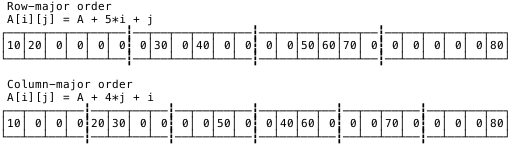
\includegraphics[width=10cm]{matrix.png}
\end{figure}

Такое представление многомерных массивов называют {\em линейным}. Оно удобно для вычислений: кроме доступа к любому элементу за $O(1)$, при итерации по строке (для row-major) или столбцу (column-major) эффективно используется кэш процессора.

\subsection*{Sparse Matrices}

Вычислительная математика часто имеет дело с {\em разреженными матрицами}, в которых подавляющая часть элементов -- нули. Представлять такие матрицы с помощью непрерывных многомерных массивов затратно: для матрицы $M\times N$ всегда будет израсходовано $\Theta(MN)$ памяти.

\subsection*{Dynamic Arrays}

\section*{Stacks}

\section*{Queues}

\subsection*{Implementation with Two Stacks}

...


\subsection*{Dynamic Maximum}

\begin{problem}
Реализовать структуру данных, в которой добавление, удаление, и вычисление максимума (или минимума) выполняется за $O(1)$
\end{problem}

Для стека задача решается добавлением ещё одного стека, на вершине которого в любой момент времени будет лежать максимум текущего стека. При удалении элемента стека последний максимум тоже удаляется.

\begin{figure}[!ht]
\centering
\includegraphics[width=6cm]{maxstack.png}
\end{figure}

Построив из двух таких стеков очередь, её максимум можно вычислить как максимум из двух вершин добавочных стеков. Итого, добавление и удаление из очереди займёт амортизированное время $O(1)$, а получение максимума -- за гарантированное $O(1)$.

\begin{problem}
Построить очередь с максимумом, в которой {\em каждое} добавление и удаление выполняется за $O(1)$
\end{problem}

\subsection*{Circular/Ring Buffers}

Рассмотренные нами массивы не позволяли эффективно реализовать очередь, для которой требуется удаление и добавление сразу в оба конца структуры данных. Это ограничение можно обойти с помощью 

\begin{figure}[!ht]
\centering
\includegraphics[width=16cm]{ringbuffer.png}
\end{figure}

%%%%%%%%%%%%%%%%%%%%%%%%%%%%%%%%%%%%%%%%%%%%%%%%%%%%%%%%%%%%%%%%%%%%%%

\section*{Linked Data Structures}

При реализации структур данных через массивы проблемы с добавлением и удалением были вызваны тем, что элементы в памяти были смежными, а размер выделенной памяти -- фиксированный.

Однако, пользуясь тем, что выделение области памяти происходит за $O(1)$, каждый элемент лежать в собственной, специально выделенной области памяти (объекте). При этом связь между объектами можно обеспечить с помощью ссылок из одних объектов на другие. Такие структуры данных называются {\em ссылочными}.

\subsection*{Linked Lists}

Простейшая из ссылочных структур данных -- {\em односвязный список} (singly-linked list). Он представляет упорядоченную последовательность элементов, каждый из которых содержит два поля: некоторое значение (payload) и ссылку, указывающую на следующий элемент, либо равную {\tt None}/{\tt null}/{\tt 0} если элемент последний в списке.

\begin{figure}[!ht]
\centering
\includegraphics[width=10cm]{linkedlist.png}
\caption{Singly-linked list}
\end{figure}

В односвязном списке доступны операции:
\begin{itemize}
  \item Добавление элемента в оба конца ($O(1)$), либо середину ($O(n)$) списка;
  \item Удаление элемента с начала ($O(1)$), либо конца ($O(n)$) списка.
\end{itemize}

При этом структура данных требует $O(n)$ дополнительной памяти для ссылок на следующие элементы.

Один из недостатков односвязного списка -- невозможность удалить элемент {\em при наличии ссылки на него}. Это решается добавлением ссылок на предыдущие элементы:

\subsection*{Double-Ended Queues (Deque)}

%!!!

%%%%%%%%%%%%%%%%%%%%%%%%%%%%%%%%%%%%%%%%%%%%%%%%%%%%%%%%%%%%%%%%%%%%%%

\section*{Sets and Dictionaries}

До этого момента мы рассматривали структуры данных с точки зрения хранения последовательности элементов, а также их добавления и удаления. Теперь к этим операциям добавится {\em поиск}.

Рассмотрим множество $K$, элементы которого будем называть {\em ключами}. На множестве ключей определена операция сравнения. Предположим для простоты, что она требует времени $O(1)$ (что, например, не выполняется для строк произвольной длины).

Необходимо представить $K$ в виде структуры данных, в которой для произвольного ключа $k$ можно эффективно проверить его принадлежность к $K$. Говорят, что такая структура реализует интерфейс {\em множества}.

Более общая задача возникает, если с каждым ключом из $K$ сопоставлены данные -- элемент из множества значений $V$.  Тогда по заданному $k$ необходимо эффективно найти соответствующий ему элемент $v \in V$. Такая структура данных реализует интерфейс {\em словаря}.



\end{document}